\begin{figure}[H]
    \renewcommand{\figurename}{Рисунок}
    \centering{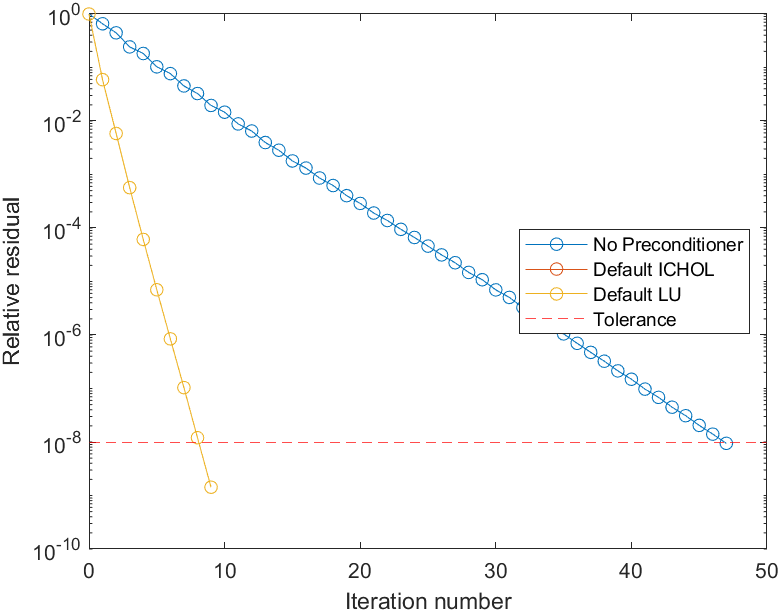
\includegraphics[scale=0.70]{img/finan512/bicg}}
    \caption{История невязок методом bicg для матрицы finan512}
    \label{fig:image_33}
\end{figure}

\begin{figure}[H]
    \renewcommand{\figurename}{Рисунок}
    \centering{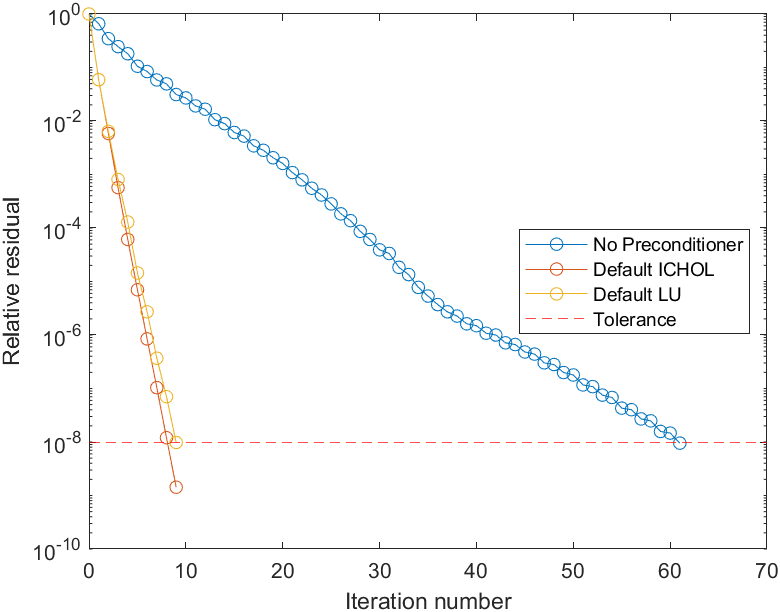
\includegraphics[scale=0.70]{img/finan512/bicgstab}}
    \caption{История невязок методом bicgstab для матрицы finan512}
    \label{fig:image_34}
\end{figure}

\begin{figure}[H]
    \renewcommand{\figurename}{Рисунок}
    \centering{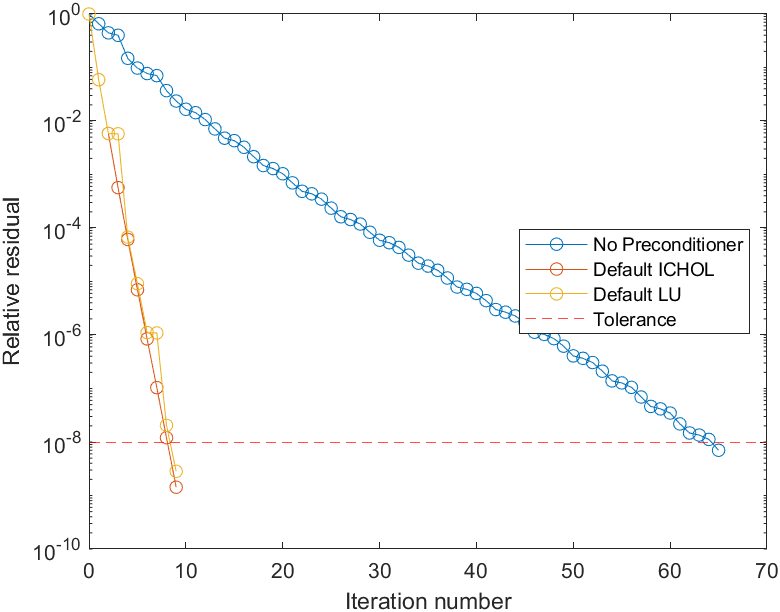
\includegraphics[scale=0.70]{img/finan512/bicgstabl}}
    \caption{История невязок методом bicgstabl для матрицы finan512}
    \label{fig:image_35}
\end{figure}

\begin{figure}[H]
    \renewcommand{\figurename}{Рисунок}
    \centering{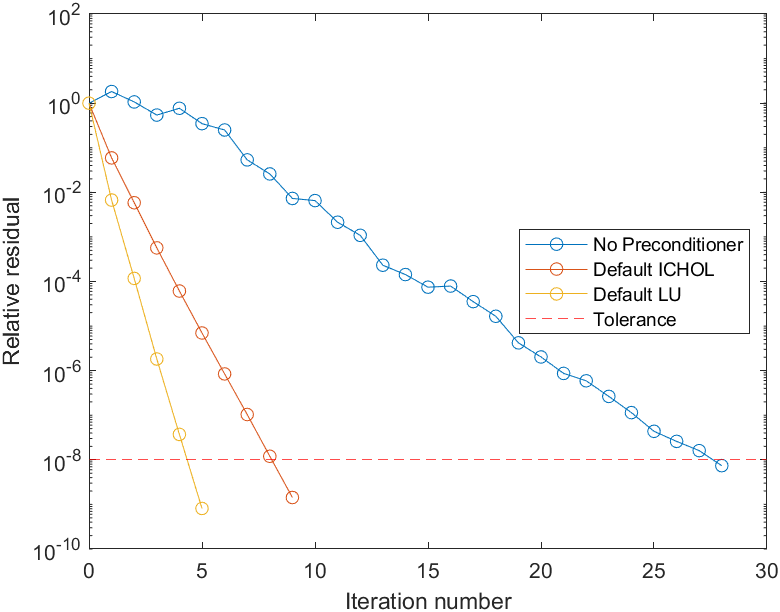
\includegraphics[scale=0.70]{img/finan512/cgs}}
    \caption{История невязок методом cgs для матрицы finan512}
    \label{fig:image_36}
\end{figure}

\begin{figure}[H]
    \renewcommand{\figurename}{Рисунок}
    \centering{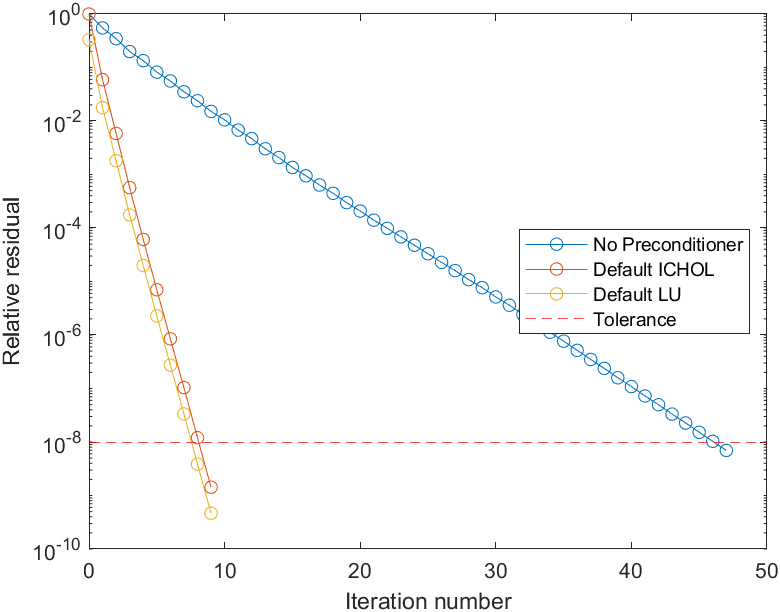
\includegraphics[scale=0.70]{img/finan512/gmres}}
    \caption{История невязок методом gmres для матрицы finan512}
    \label{fig:image_37}
\end{figure}

\begin{figure}[H]
    \renewcommand{\figurename}{Рисунок}
    \centering{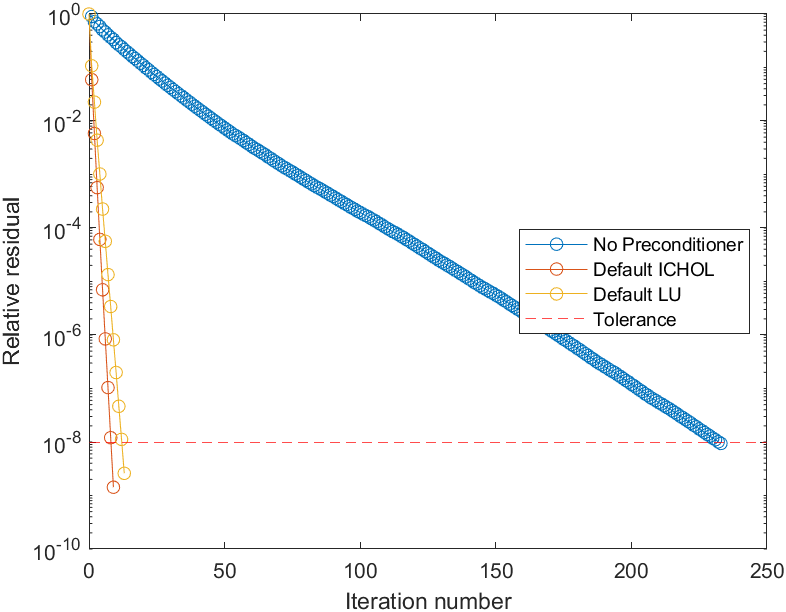
\includegraphics[scale=0.70]{img/finan512/lsqr}}
    \caption{История невязок методом lsqr для матрицы finan512}
    \label{fig:image_38}
\end{figure}

\begin{figure}[H]
    \renewcommand{\figurename}{Рисунок}
    \centering{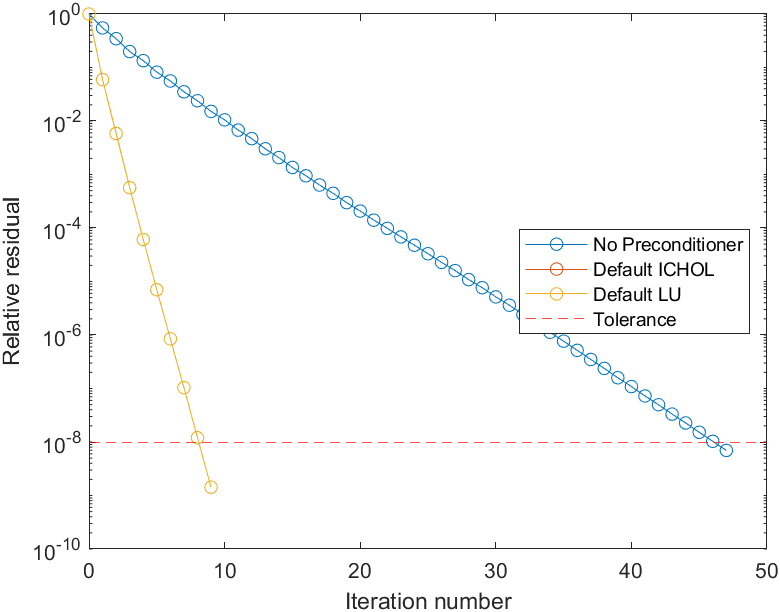
\includegraphics[scale=0.70]{img/finan512/minres}}
    \caption{История невязок методом minres для матрицы finan512}
    \label{fig:image_39}
\end{figure}

\begin{figure}[H]
    \renewcommand{\figurename}{Рисунок}
    \centering{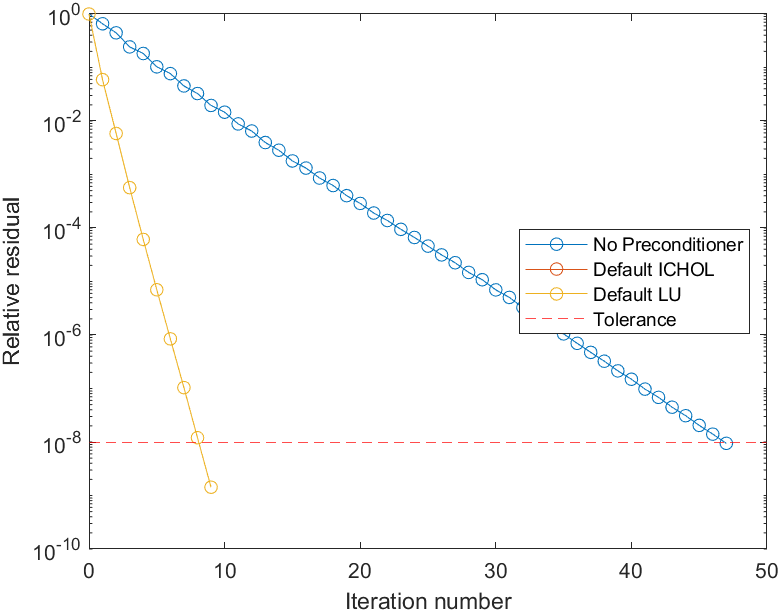
\includegraphics[scale=0.70]{img/finan512/pcg}}
    \caption{История невязок методом pcg для матрицы finan512}
    \label{fig:image_40}
\end{figure}

\begin{figure}[H]
    \renewcommand{\figurename}{Рисунок}
    \centering{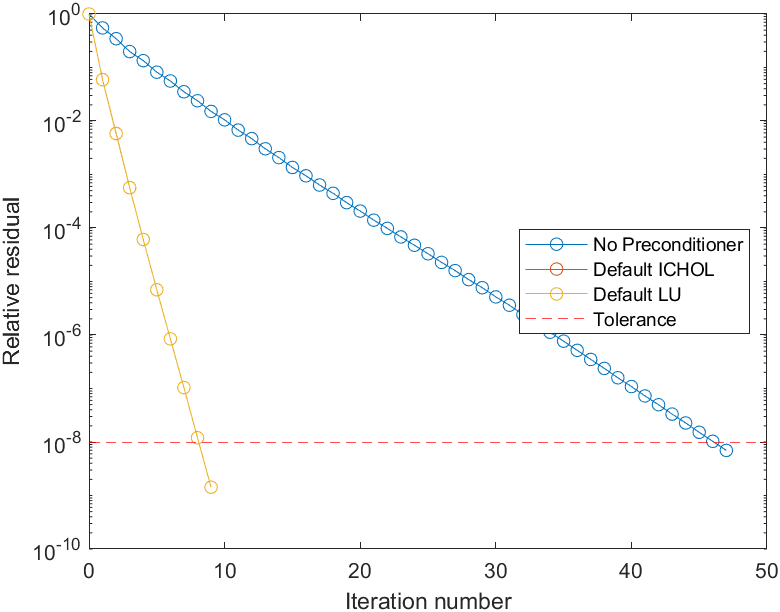
\includegraphics[scale=0.70]{img/finan512/qmr}}
    \caption{История невязок методом qmr для матрицы finan512}
    \label{fig:image_41}
\end{figure}

\begin{figure}[H]
    \renewcommand{\figurename}{Рисунок}
    \centering{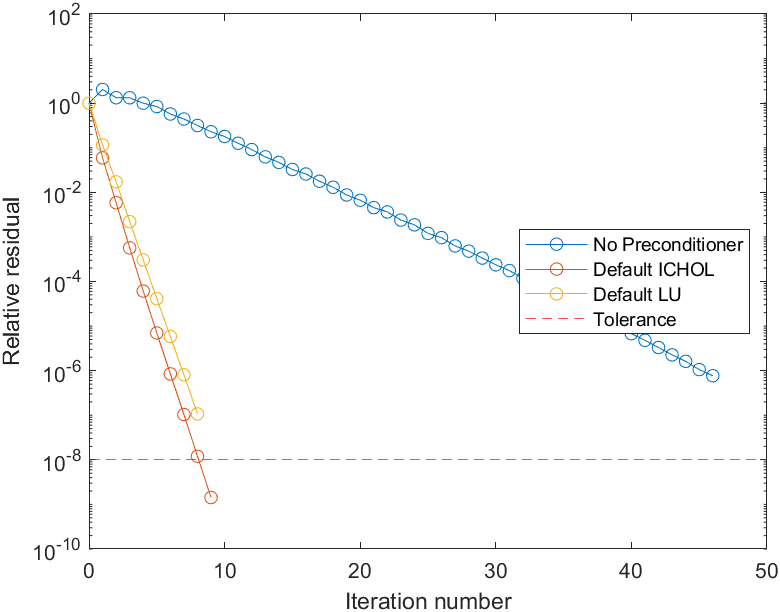
\includegraphics[scale=0.70]{img/finan512/symmlq}}
    \caption{История невязок методом symmlq для матрицы finan512}
    \label{fig:image_42}
\end{figure}

\begin{figure}[H]
    \renewcommand{\figurename}{Рисунок}
    \centering{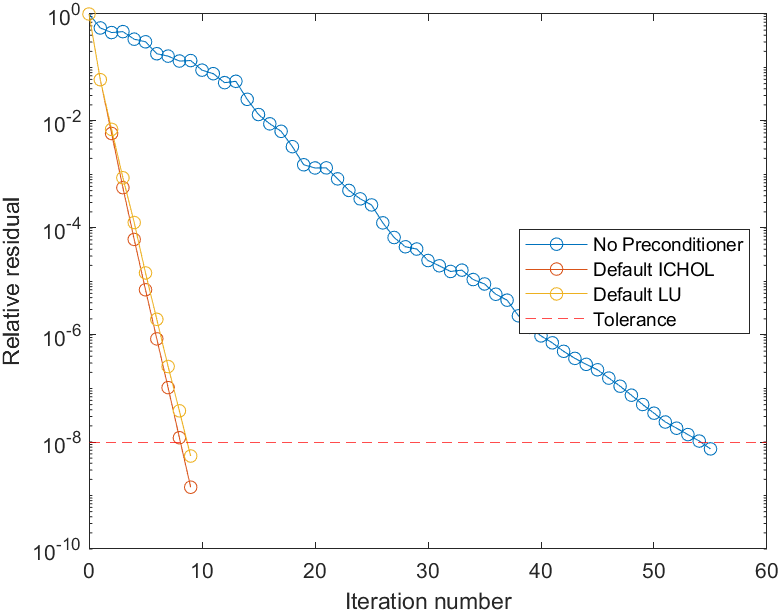
\includegraphics[scale=0.70]{img/finan512/tfqmr}}
    \caption{История невязок методом tfqmr для матрицы finan512}
    \label{fig:image_43}
\end{figure}